% !TeX program = pdflatex
% =============================================================================
% Klasse 4fh: Reproduktion des an 4fh abgegebenen PDFs
% Vorlage: Klasse-fh/aufgabenblatt3-kondensatoren-teil1.pdf (24.08.2026, mit
% Loesungen), eingesetzt in der 4fh am 25.08.2026.
%
% Diese Fassung ist AELTER als aufgabenblatt3-kondensatoren.tex im
% Themenordner (Umbau am 27.08.2026 vor der 4cdeg-Lektion). Unterschiede zum
% heutigen Stand: farbiges Box-Layout, keine Excel-Hinweisbox, Teil 1(a) fragt
% direkt nach Q = C*U, Teil 2(c) enthaelt die algebraische Herleitung der
% Kondensatorformel (heute im Plenum des Arbeitsblatts), Teil 2(d) mit der
% eps0-Abweichung aus der Excel-Vorlage, keine Loesungsbilder (Excel-
% Screenshots). Text aus dem 4fh-PDF rekonstruiert.
% =============================================================================
\documentclass[addpoints,11pt,a4paper]{exam}

\usepackage[T1]{fontenc}
\usepackage[utf8]{inputenc}
\usepackage[ngerman]{babel}
\usepackage{lmodern}
\usepackage[a4paper,margin=2.2cm,headheight=14pt]{geometry}
\usepackage{amsmath}
\usepackage{siunitx}
\sisetup{per-mode=fraction,fraction-command=\frac}
\usepackage{array,booktabs,tabularx,multirow}
\usepackage{enumitem}
\usepackage{xcolor}
\usepackage{colortbl}
\usepackage{tikz}
\usepackage{physics}
\usepackage{circuitikz}
\usepackage[most]{tcolorbox}
\usepackage{lastpage}
\usepackage{graphicx}
% Bilder liegen im uebergeordneten Themenordner (nicht dupliziert).
\graphicspath{{../}}
\usepackage{hyperref}

\usetikzlibrary{arrows.meta,calc,angles,quotes}

\usepackage{setspace}
\usepackage{needspace}
\setlength{\parindent}{0pt}
\setlength{\parskip}{0.6em}
\setstretch{1.08}
\setlist[itemize]{itemsep=0.4em}

% -----------------------------
% Farben (Corporate-Farbschema Physik KFR)
% -----------------------------
\definecolor{titleblue}{HTML}{183A6B}
\definecolor{accentblue}{HTML}{2E6F9E}
\definecolor{lightblue}{HTML}{EAF4FB}
\definecolor{verylightblue}{HTML}{F7FBFE}
\definecolor{lightgray}{HTML}{F4F6F8}
\definecolor{darkgray}{HTML}{4A4A4A}
\definecolor{accentorange}{HTML}{D9720C}
\definecolor{accentpurple}{HTML}{7B2D8E}
\definecolor{theorygreen}{HTML}{2E7D4F}
\definecolor{lighttheorygreen}{HTML}{EAF7EF}
\definecolor{groupteal}{HTML}{1B7F72}
\definecolor{lightgroupteal}{HTML}{E8F5F3}
\definecolor{lightorange}{HTML}{FCEEE0}

\hypersetup{
  colorlinks=true,
  urlcolor=accentblue,
  linkcolor=accentblue,
  pdftitle={Aufgabenblatt 3: Kondensatoren},
  pdfauthor={Loris Keller}
}

\newcolumntype{Y}{>{\centering\arraybackslash}X}
\newcolumntype{P}[1]{>{\raggedright\arraybackslash}p{#1}}

% -----------------------------
% Boxen (farbiges Layout, Stand 4fh vor der Umstellung vom 31.08.2026)
% -----------------------------
\tcbset{before skip=10pt, after skip=10pt}
\newtcolorbox{titlebox}{
  enhanced,
  colback=titleblue,
  colframe=titleblue,
  boxrule=0pt,
  arc=3mm,
  left=3mm,right=3mm,top=3mm,bottom=3mm
}

\newlength{\aufgabenindent}
\settowidth{\aufgabenindent}{10.\hskip\labelsep}

\newtcolorbox{infobox}{
  enhanced,
  breakable,
  colback=lightblue,
  colframe=accentblue,
  boxrule=0.7pt,
  arc=2mm,
  left=6mm,right=6mm,top=3.5mm,bottom=3.5mm
}

\newtcolorbox{theoriebox}[1][Theorie]{
  enhanced,
  breakable,
  colback=lighttheorygreen,
  colframe=theorygreen,
  title={#1},
  fonttitle=\bfseries,
  boxrule=0.7pt,
  arc=2mm,
  left=6mm,right=6mm,top=3.5mm,bottom=3.5mm
}

\newtcolorbox{beispielbox}[1][Beispiel]{
  enhanced,
  breakable,
  colback=verylightblue,
  colframe=accentblue,
  title={#1},
  fonttitle=\bfseries,
  boxrule=0.7pt,
  arc=2mm,
  left=6mm,right=6mm,top=3.5mm,bottom=3.5mm
}

\newtcolorbox{groupbox}[1][Gruppenarbeit]{
  enhanced,
  breakable,
  colback=lightgroupteal,
  colframe=groupteal,
  title={#1},
  fonttitle=\bfseries,
  boxrule=0.7pt,
  arc=2mm,
  enlarge left by=-\aufgabenindent,
  width=\textwidth,
  left=6mm,right=6mm,top=3.5mm,bottom=3.5mm
}

\newtcolorbox{hinweisbox}[1][Hinweis]{
  enhanced,
  breakable,
  colback=lightorange,
  colframe=accentorange,
  title={#1},
  fonttitle=\bfseries,
  boxrule=0.7pt,
  arc=2mm,
  left=6mm,right=6mm,top=3.5mm,bottom=3.5mm
}


% teilkopf: farbiger Zwischentitel (Petrol) fuer die Teile 1-4 der Lernaufgabe.
\newtcolorbox{teilkopf}{
  enhanced,
  colback=groupteal,
  colframe=groupteal,
  coltext=white,
  boxrule=0pt,
  arc=1.5mm,
  left=4mm,right=4mm,top=1.5mm,bottom=1.5mm,
  before skip=8pt, after skip=6pt,
  fontupper=\bfseries\sffamily
}

% Marke: kleines farbiges Inline-Label (z.B. "Eure Kondensatorformel").
\newtcbox{\Marke}[1][accentpurple]{
  nobeforeafter,
  colback=#1,
  colframe=#1,
  coltext=white,
  boxrule=0pt,
  arc=2pt,
  left=5pt,right=5pt,top=2pt,bottom=2pt,
  fontupper=\bfseries\sffamily\small
}

\newtcolorbox{answerbox}{
  breakable,
  colback=white,
  colframe=gray!55,
  boxrule=0.5pt,
  arc=1.5mm,
  left=2mm,right=2mm,top=2mm,bottom=2mm
}

% --- Lösungen ein-/ausblenden -----------------------------------------------
% Schuelerversion (Standard):  pdflatex <name>.tex
% Loesungsversion:             pdflatex -jobname=<name>_Loesung "\def\MitLoesung{}\input{<name>}"
\ifdefined\MitLoesung\printanswers\else\noprintanswers\fi

\pointformat{}
\renewcommand{\solutiontitle}{\noindent\color{titleblue}\textbf{Lösung:}\enspace}

\pagestyle{headandfoot}
\cfoot{\textcolor{darkgray}{Seite \thepage\ von \pageref{LastPage}}}

\newcommand{\Kopfzeile}[4]{%
  \begin{titlebox}
    {\color{white}\sffamily\bfseries\Large #4}
  \end{titlebox}
  \vspace{0.5em}
  \noindent\textbf{Klasse:}~#1 \hfill \textbf{Datum:}~#2 \hfill \textbf{Thema:}~#3
    \hfill \textbf{Lehrperson:}~Loris Keller
  \vspace{0.8em}
  \lhead{\textcolor{darkgray}{#3}}
  \rhead{\textcolor{darkgray}{#4}}
}

\newlength{\antwortraumlen}
\newcommand{\Antwortraum}[1]{%
  \pgfmathsetlength{\antwortraumlen}{#1*2.5cm}%
  \begin{answerbox}
    \rule{0pt}{\antwortraumlen}%
  \end{answerbox}%
}

% Werte für Kopfzeile zentral setzen (wie im 4fh-PDF)
\newcommand{\Klasse}{4fh / 4cdeg (SP4)}
\newcommand{\Datum}{25.08.2026 (4fh) / 28.08.2026 (4cdeg)}
\newcommand{\Thema}{Kondensatoren}
\newcommand{\ArbeitsblattTitel}{Aufgabenblatt 3: Kondensatoren}

\begin{document}

\Kopfzeile{\Klasse}{\Datum}{\Thema}{\ArbeitsblattTitel}

% =============================================================================
% Lernaufgabe
% =============================================================================
\begin{questions}
\begin{groupbox}[Lernaufgabe (Partnerarbeit): Kapazität mit der PhET-Simulation bestimmen]
\noindent
\begin{minipage}[c]{1.8cm}
  \href{https://phet.colorado.edu/de/simulations/capacitor-lab-basics}{%
    
\includegraphics[width=1.6cm]{Bilder/phet-logo-trademarked.png}}
\end{minipage}%
\begin{minipage}[c]{\dimexpr\linewidth-1.8cm\relax}
Öffnen Sie zu zweit die Simulation
\href{https://phet.colorado.edu/de/simulations/capacitor-lab-basics}{\glqq Capacitor Lab: Basics\grqq{}}.
\end{minipage}

\begin{center}
  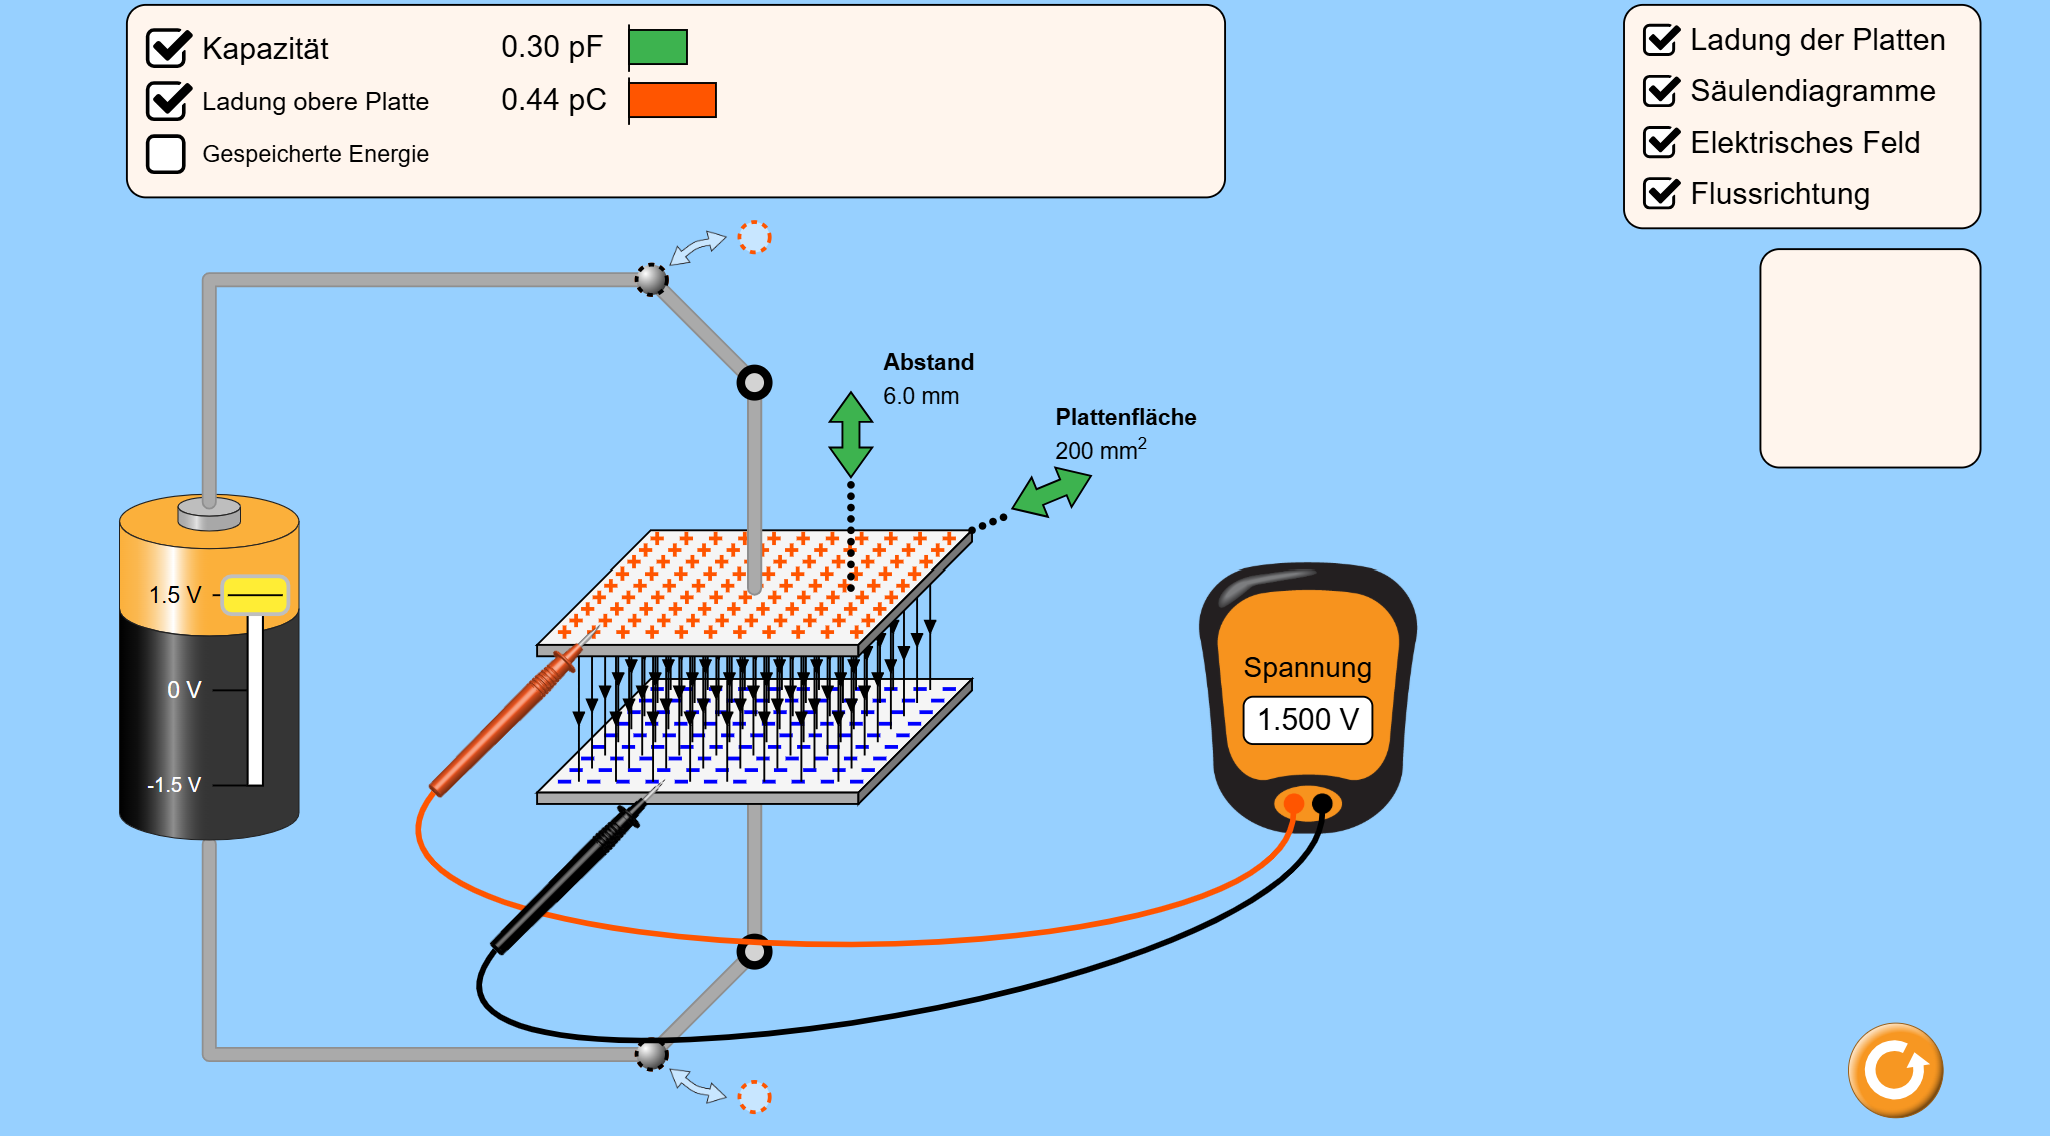
\includegraphics[width=10cm]{Bilder/Phet_Kapazitaet.png}
\end{center}
{\scriptsize So sieht der Einstiegsscreen der Simulation aus: Links die
Anzeigen für Kapazität und Ladung, in der Mitte der Plattenkondensator mit
verstellbarer Plattenfläche und verstellbarem Abstand, rechts das
Multimeter für die Spannung.}

\noindent
\begin{minipage}[c]{1.3cm}
  
\includegraphics[width=1.1cm]{Bilder/excel_logo.jpg}
\end{minipage}%
\begin{minipage}[c]{\dimexpr\linewidth-2.4cm\relax}
Öffnen Sie ausserdem die vorbereitete Excel-Vorlage
\texttt{kondensatoren-phet-\allowbreak messvorlage.xlsx} für Ihre Messwerte.
\end{minipage}

% -----------------------------------------------------------------------------
\question
\begin{teilkopf}
Teil 1: Zusammenhang zwischen $Q$, $U$ und $C$
\end{teilkopf}
Halten Sie die Geometrie des Plattenkondensators (Fläche $A$, Abstand $d$)
konstant. Verändern Sie die angelegte Spannung $U$ in mehreren Schritten
und lesen Sie jeweils die Ladung $Q$ ab. Tragen Sie Ihre Messwerte in die
Excel-Vorlage ein, erstellen Sie ein $U$-$Q$-Diagramm und fügen Sie eine
Trendlinie ein.
\begin{parts}
  \needspace{14cm}
  \part[4] Welchen Funktionstyp erwarten Sie für den Zusammenhang zwischen
  $Q$ und $U$, und wie äussert sich das im Diagramm? Was entspricht die
  Steigung der Trendlinie physikalisch, und welche Gleichung für den
  Zusammenhang zwischen $Q$, $C$ und $U$ folgt daraus?
  \Antwortraum{4}
  \begin{solution}
  Einen linearen, proportionalen Zusammenhang ($Q\sim U$): Die Messpunkte
  liegen auf einer Ursprungsgeraden. Die Steigung der Trendlinie
  entspricht der Kapazität $C$ des eingestellten Kondensators. Da $Q$
  proportional zu $U$ ist mit Proportionalitätsfaktor $C$, folgt:
  $Q=C\cdot U$.
  \end{solution}

  \part[2] Vergleichen Sie die abgelesene Kapazität mit dem Wert, den die
  Simulation direkt anzeigt. Stimmen die Werte überein?
  \Antwortraum{2}
  \begin{solution}
  Ja, die aus der Steigung der Trendlinie abgelesene Kapazität sollte (im
  Rahmen der Ablesegenauigkeit) mit dem von der Simulation angezeigten Wert
  übereinstimmen. Das bestätigt, dass die Steigung der Trendlinie
  tatsächlich der Kapazität $C$ entspricht.
  \end{solution}
\end{parts}

% -----------------------------------------------------------------------------
\question
\begin{teilkopf}
Teil 2: Einfluss von Fläche und Abstand
\end{teilkopf}
Untersuchen Sie jetzt, wie die Kapazität von der Geometrie abhängt.
\begin{parts}
  \part[3] Halten Sie den Plattenabstand $d$ konstant und notieren Sie
  seinen Wert in der dafür vorgesehenen Zelle der Excel-Vorlage. Verändern
  Sie die Plattenfläche $A$. Tragen Sie die Werte in ein $A$-$C$-Diagramm
  ein, fügen Sie eine Trendlinie ein und beschreiben Sie den Zusammenhang.
  \Antwortraum{3}
  \begin{solution}
  $C$ wächst proportional zu $A$ (Ursprungsgerade im $A$-$C$-Diagramm, bei
  konstantem $d$): $C \sim A$.
  \end{solution}

  \part[3] Halten Sie nun die Plattenfläche $A$ konstant und notieren Sie
  ihren Wert in der dafür vorgesehenen Zelle der Excel-Vorlage. Verändern
  Sie den Plattenabstand $d$. Tragen Sie die Werte in ein $d$-$C$-Diagramm
  ein, fügen Sie eine Trendlinie ein und beschreiben Sie den Zusammenhang.
  \Antwortraum{3}
  \begin{solution}
  $C$ nimmt mit wachsendem $d$ ab, und zwar umgekehrt proportional:
  $C \sim \frac{1}{d}$ (bei konstantem $A$).
  \end{solution}

  \part[6] Kombinieren Sie Ihre Resultate aus den beiden vorherigen
  Teilaufgaben mit den im Arbeitsblatt 4 (Theorie 2) repetierten Formeln
  $E=\dfrac{Q}{\varepsilon_0\cdot A}$ und $U=E\cdot d$, um algebraisch
  herzuleiten, wovon die Kapazität $C$ genau abhängt. Zeigen Sie Ihren
  vollständigen Rechenweg.
  \Antwortraum{6}
  \begin{solution}
  $U=E\cdot d$ mit $E=\dfrac{Q}{\varepsilon_0\cdot A}$ eingesetzt:
  \[
    U = \frac{Q}{\varepsilon_0\cdot A}\cdot d.
  \]
  Mit $\varepsilon_0\cdot A$ multiplizieren:
  \[
    U\cdot\varepsilon_0\cdot A = Q\cdot d.
  \]
  Durch $d$ dividieren, nach $Q$ aufgelöst:
  \[
    Q = U\cdot\frac{\varepsilon_0\cdot A}{d}.
  \]
  Vergleich mit $Q=C\cdot U$ aus Teil 1: Der Vorfaktor von $U$ muss die
  Kapazität sein:
  \[
    \boxed{C = \frac{\varepsilon_0\cdot A}{d}}.
  \]
  Das bestätigt auch die aus den eigenen Messdaten gefundenen
  Zusammenhänge $C\sim A$ und $C\sim\frac{1}{d}$.
  \end{solution}

  \Marke[accentorange]{Eure Kondensatorformel} (kein Punkteanteil, bitte
  trotzdem in eigener Handschrift eintragen):
  \Antwortraum{1}
  \begin{solution}
  \[
    C = \varepsilon_0\cdot\frac{A}{d}.
  \]
  \end{solution}

  \part[3] Die Excel-Vorlage berechnet aus euren Messwerten in den
  Tabellenblättern \glqq Teil 2a\grqq{} und \glqq Teil 2b\grqq{}
  automatisch je einen Mittelwert für $\varepsilon_0$ (unterhalb der
  Messtabelle). Notieren Sie beide Werte und berechnen Sie die relative
  Abweichung vom Literaturwert
  $\varepsilon_0\approx\SI{8.85e-12}{\farad\per\meter}$ in Prozent. Nennen
  Sie ausserdem eine mögliche Fehlerquelle dafür (Tipp: Was wird bei der
  Herleitung der Formel vernachlässigt? Siehe Theorie 2 im Arbeitsblatt 4).
  \Antwortraum{3}
  \begin{solution}
  Relative Abweichung:
  \[
    \left|\frac{\varepsilon_{0,\text{gemessen}}-\varepsilon_0}{\varepsilon_0}\right|\times\SI{100}{\percent}.
  \]
  Die gemessenen Mittelwerte sollten nur um wenige Prozent vom
  Literaturwert abweichen. Mögliche Fehlerquellen: Ablesegenauigkeit in der
  Simulation, oder die bei der Herleitung vernachlässigten Randeffekte des
  elektrischen Feldes an den Plattenrändern (siehe Hinweisbox in Theorie 2
  im Arbeitsblatt).
  \end{solution}
\end{parts}

% -----------------------------------------------------------------------------
\question
\begin{teilkopf}
Teil 3: Kondensator von der Batterie getrennt
\end{teilkopf}
Laden Sie den Kondensator wie in Teil 1 auf und trennen Sie ihn danach von
der Batterie (Schalter in der Simulation öffnen).
\begin{parts}
  \part[2] Verändern Sie nun den Plattenabstand $d$. Welche Grösse bleibt
  dabei konstant, welche ändert sich? Begründen Sie mit $Q=C\cdot U$.
  \Antwortraum{2}
  \begin{solution}
  Da der Kondensator von der Spannungsquelle getrennt ist, kann keine
  Ladung mehr zu- oder abfliessen: Die Ladung $Q$ bleibt konstant. Der
  Plattenabstand $d$ verändert dagegen die Kapazität
  $C=\varepsilon_0\cdot\frac{A}{d}$, also muss sich gemäss $Q=C\cdot U$
  die Spannung $U$ anpassen.
  \end{solution}

  \part[2] Was passiert konkret mit der Spannung $U$, wenn Sie $d$
  vergrössern? Überprüfen Sie Ihre Vorhersage in der Simulation.
  \Antwortraum{2}
  \begin{solution}
  Wird $d$ vergrössert, so wird $C$ kleiner (da $C\sim\frac{1}{d}$). Weil
  $Q$ konstant bleibt, muss $U=\frac{Q}{C}$ steigen: Die Spannungsanzeige
  der Simulation nimmt zu.
  \end{solution}
\end{parts}

% -----------------------------------------------------------------------------
\question[3]
\begin{teilkopf}
Teil 4: Leuchtdauer im Simulationsscreen \glqq Light Bulb\grqq{}
\end{teilkopf}
Wechseln Sie zum zweiten Screen der Simulation, wo der Kondensator statt an
eine Batterie an eine Glühbirne angeschlossen ist.
\begin{center}
  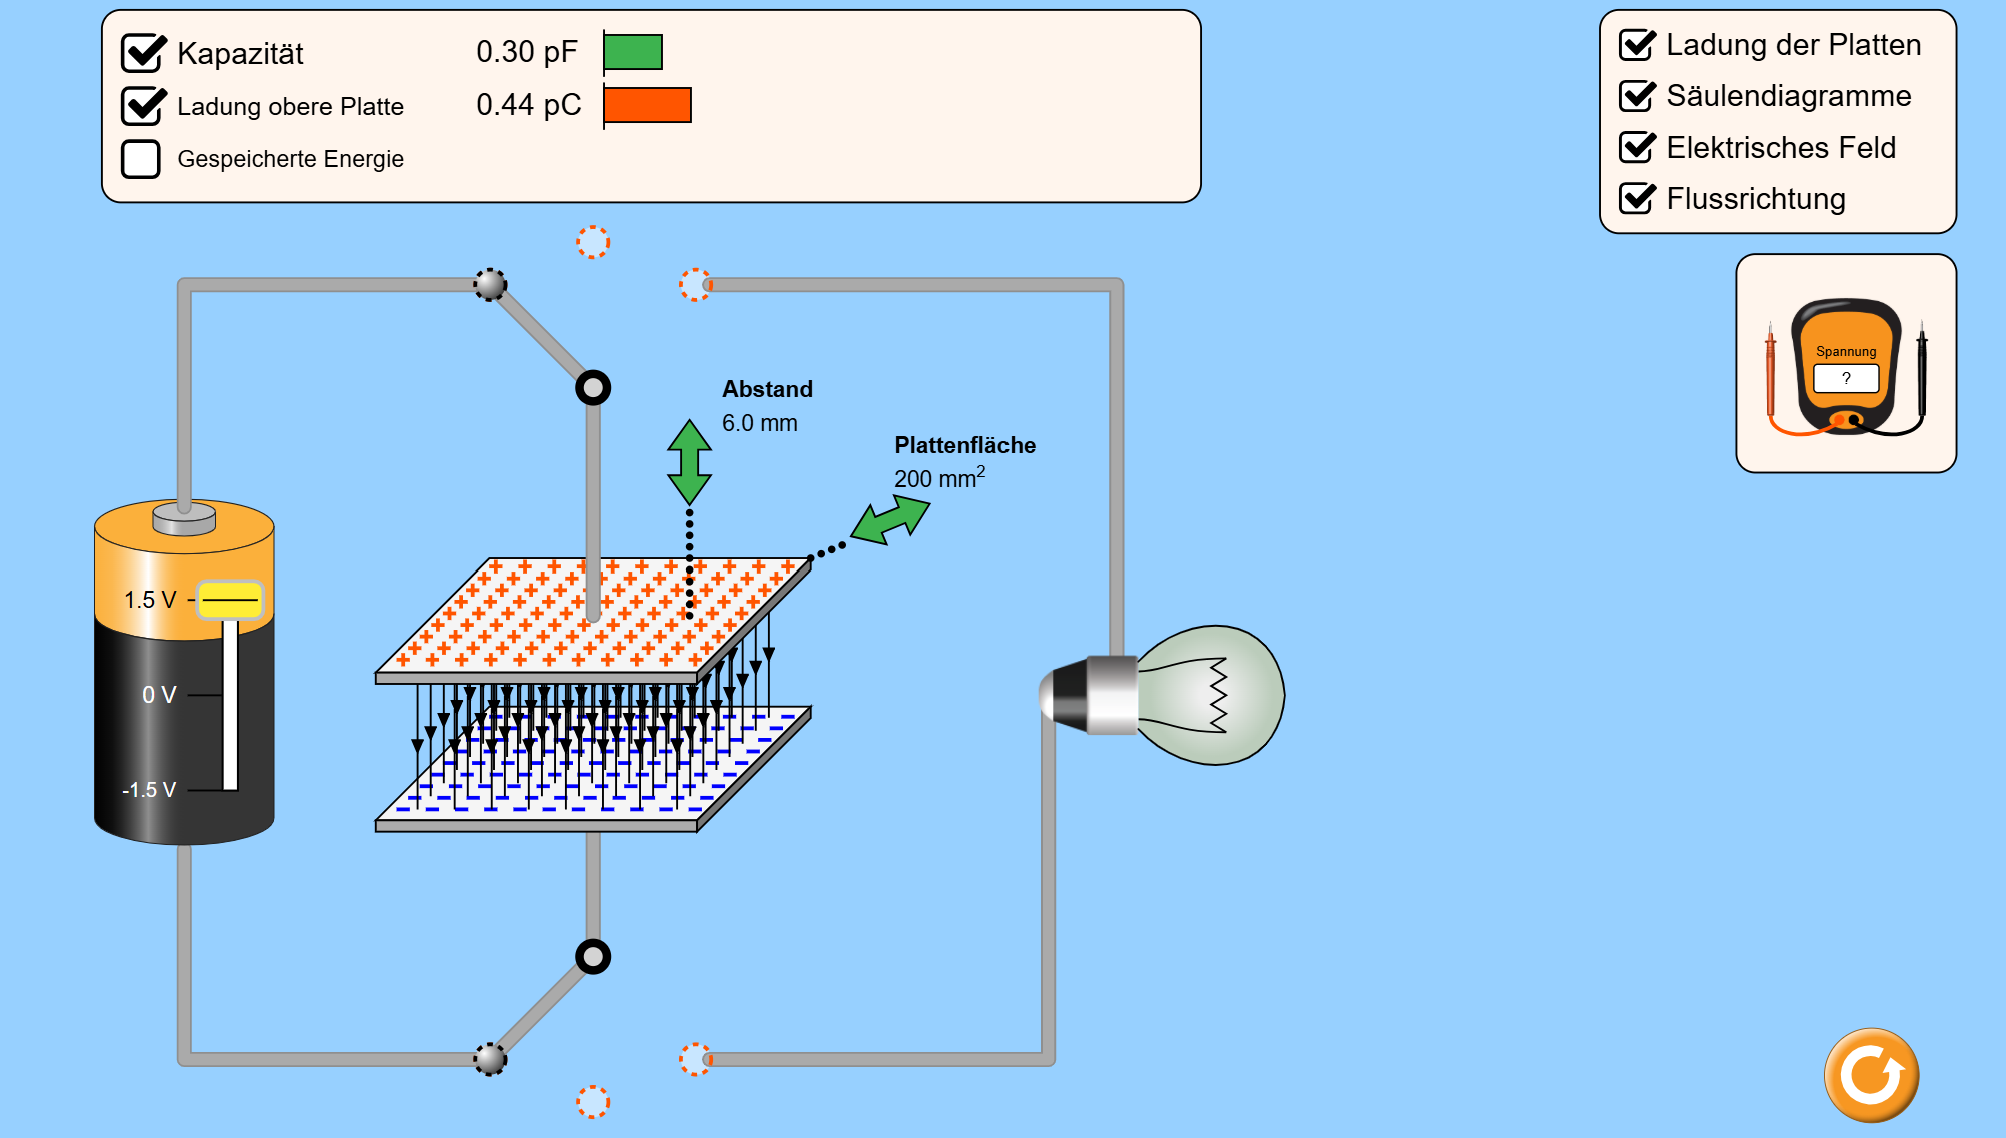
\includegraphics[width=9cm]{Bilder/Phet_Lichtquelle.png}
\end{center}
{\scriptsize Der Screen \glqq Light Bulb\grqq{}: Batterie, Kondensator und
Glühbirne im selben Stromkreis.}

Laden Sie zwei Kondensatoren mit unterschiedlicher Kapazität (z.\,B. über
die Plattenfläche $A$) bei derselben Spannung $U$, trennen Sie sie danach
von der Batterie und lassen Sie sie über die Glühbirne entladen. Bestätigen
Sie damit Ihre Vorhersage aus dem Demoversuch, und begründen Sie
zusätzlich mit $Q=C\cdot U$, weshalb der Kondensator mit der grösseren
Kapazität mehr Ladung enthält.
\Antwortraum{3}
\begin{solution}
Wie im Demoversuch vorhergesagt, leuchtet die Glühbirne beim Kondensator
mit grösserer Kapazität länger. Da $U$ bei beiden Kondensatoren gleich
ist, folgt aus $Q=C\cdot U$ direkt: Ein grösseres $C$ bedeutet ein
grösseres $Q$, also mehr Ladung, die über die Glühbirne abfliessen muss.
\end{solution}
\end{groupbox}
\end{questions}

\end{document}
